\documentclass[12pt]{article}
\usepackage[utf8]{inputenc}
\usepackage[francais]{babel}
\usepackage{amsthm}
\usepackage{geometry}
\usepackage{graphicx}
\usepackage{fancyhdr}
\usepackage{hyperref}
\hypersetup{
    colorlinks,
    citecolor=black,
    filecolor=black,
    linkcolor=black,
    urlcolor=black
}

\geometry{hmargin=2cm, vmargin=2cm}

\def\blurb{Linköping University\\
IDA - The Department of Computer and Information Science}


\def\ligne#1{%
  \hbox to \hsize{%
    \vbox{\centering #1}}}%

\makeatletter
\def\maketitle{%
	\null
	\vfill
	\vbox{\centering \Large \textbf{\blurb}}
	\vspace{15mm}
	\vbox{\centering \LARGE \textbf{\@title}}
	\vspace{15mm}
	\vbox{\centering \@author}
	\vspace{8mm}
	\vbox{\centering \@date}
	\vfill
}

\title{TDDC17 - Lab 4 : Bayesian Networks}
\author{Simon Vernhes \texttt{<simon@vernhes.eu>}}
\date{\today}

\begin{document}
  \pagestyle{fancyplain}
  \setlength{\parskip}{.6ex plus .4ex minus .4ex}
  \renewcommand{\headrulewidth}{0pt}
  \renewcommand{\footrulewidth}{0.6pt}
  \fancyhf{}
  \fancyhead{} 
  \lfoot{\@title \\ \@author}
  \rfoot{Page \thepage}
  \maketitle \clearpage
  
  \section{Querying an existing network}
  \subsection{Question 1}
The risk of meltdown during a day if no observations have been made is $0.0.2578$. If there's icy weather, the risk of meltdown is $0.03472$.

  \subsection{Question 2}
Both warning sensors indicate failure : $P(meltdown | pumpFailureWarning, waterLeakWarning) = 0.14535$. Actual pump failure and water leak : $P(meltdown | pumpFailure, waterLeak) = 0.2$.

  \subsection{Question 3}

Sometimes it's very difficult or impossible to make repeated experiments or observation. So it's become very difficult to get accurate numbers for conditional probabilities for some stochastic variables.

For this example, it may be difficult to know the risk of meltdown give a pump failure or/and a water leak.

  \subsection{Question 4}
The domain for variable Temperature could be :
\begin{itemize}
  \item continuous random variable : $[-273 ; +\infty]$ 
  \item discrete random variable : $\left\{EXTREMELY\_COLD, VERY\_COLD, COLD, NORMAL, HOT, VERY\_HOT, EXTREMELY\_HOT\right\}$
\end{itemize}

For the continuous random variable, $P(waterLeak | Temperature)$ may have high probabilities when near $-273^oC$ and decreasing while temperature increase. 

For the discrete random variable, the probability distribution could be as follow :

\begin{tabular}{|c|c|c|}
  \hline
  Temperature & $P(\lnot waterLeak | Temperature)$
                                  & $P(waterLeak | Temperature)$ \\ \hline
  $EXTREMELY\_COLD$  & 0.30 & 0.70  \\ \hline
  $VERY\_COLD$       & 0.35 & 0.65  \\ \hline
  $COLD$             & 0.40 & 0.60  \\ \hline
  $NORMAL$           & 0.50 & 0.50  \\ \hline
  $HOT$              & 0.80 & 0.20  \\ \hline
  $VERY\_HOT$        & 0.95 & 0.05  \\ \hline
  $EXTREMELY\_HOT$   & 0.99 & 0.01  \\ \hline
\end{tabular}



  \section{Extending a network}

  \subsection{Question 1}
If the radio doesn't work : $P(survives | \lnot rdaio) = 0.98116$. The probability is still high because the probability of meltdown is low and because if the radio doesn't that not necessarily means that the battery is dead.

  \subsection{Question 2}
\textbf{We know :}

$P(bicycle\_works) = 0.9$

$P(survives | \lnot moves \land meltdown \land bicycle\_works) = 0.6$

$P(survives | moves \land meltdown \land bicycle\_works) = 0.9$

\textbf{So :}

$P(survives) = P(bicycle\_works) \* P(survives | bicycle\_works) + P(\lnot bicycle\_works) \* P(survives | \lnot bicycle\_works)$

\textbf{But :}

$P(survives | \lnot bicycle\_works = 0$

\textbf{And :}

$P(survives | bicycle\_works) = P(meltdown) \* P(survives | bicycle\_works \land meltdown) + P(\lnot meltdown) \* P(survives | bicycle\_world \land \lnot meltdown)
$

\textbf{But :}

$P(survives | bicycle\_world \land \lnot meltdown) = 1$

\textbf{And :}

$P(survives | bicycle\_works \land  meltdown) =  P(\lnot moves) \* P(survives | \lnot moves \land meltdown \land bicycle\_works) + P(moves) \* P(survives | moves \land meltdown \land bicycle\_works)$

\textbf{So :}

$P(survives) = P(bicycle\_works) \* (P(meltdown) \* (P(\lnot moves) \* P(survives | \lnot moves \land meltdown \land bicycle\_works) + P(moves) \* P(survives | moves \land meltdown \land bicycle\_works)) + P(\lnot meltdown))$ 

$\Leftrightarrow P(survives) = 0.9 \* (0.03 \* (0.6\*P(\lnot moves) + 0.9\*P(moves)) + 0.97)$

\textbf{If we suppose that } $P(moves) = 0.95$ \textbf{then :}

$P(survives) = 0.889605$

  \subsection{Question 3}

The complexity of exact inference in Bayesian networks, using variable elimination is exponential. We know that for exact inference in Bayesian networks ($X$ query variable, $E$ evidence variable, $Y$ unobserved variable) :

$P(X | e) = \alpha \* P(X, e) = \alpha\*\sum_{y} P(X, e, y)$

So if there is n unobserved variable :

$P(X | e) = \alpha \* \sum_{Y \in \{Y_1, Y_2, ..., Y_n\}} \sum_{y \in Y} P(X, e, y)$

So, the complexity of exact inference is the multiplication of the number of event of each unobserved. So for boolean stochastic variable : $O(2^n)$


  \section{More extensions}

  \subsection{Question 1}

In my model, replacing the pump by a better one just means changing the probabilities of PumpFailure (decreasing the probability of failure). 

  \subsection{Question 2}

\textbf{Let} $s = survives$ ; $pfw = pumpFailureWarning$ and $wlw = waterLeakWarning$

$P(s | pfw \lor wlw) = \frac{P(s \land (pfw \lor wlw))}{P(pfw \lor wfw)}
  = \frac{P((s \land pfw) \lor (s \land wlw))}{P(pfw \lor wfw)}$

Or we can easily assume that $WaterLeak$ and $PumpFailure$ are independent and so the warning. \textbf{So :}

$P(s | pfw \lor wlw) = \frac{P(s \land pfw) + P(s \land wlw) - P(s \land pfw \land wlw)}{P(pfw) + p(wlw) - P(pfw)\*P(wlw)}
  = \frac{P(s|pfw)\*P(pfw) + P(s|wlw)\*P(wlw) - P(s|pfw \land wlw)\*P(pfw \land wlw)}{P(pfw) + p(wlw) - P(pfw)\*P(wlw)}$

\textbf{Finally :}

$P(s | pfw \lor wlw)  = \frac{P(s|pfw)\*P(pfw) + P(s|wlw)\*P(wlw) - P(s|pfw \land wlw)\*P(pfw)\*P(wlw)}{P(pfw) + p(wlw) - P(pfw)\*P(wlw)}$

\textbf{The chance of survives is :}
$P(s | pfw \lor wlw)  = \frac{0.96*0.14 + 0.97*0.14 - 0.94*0.14*0.14}{0.14 + 0.14 - 0.14*0.14} = 0.96688$

  \subsection{Question 3}

When we create a Bayesian Network model of a person we restrict the person at a limited set of action which is unrealistic for a person.

  \subsection{Question 4}

To model a more dynamic world where \texttt{IcyWeather} is more likely to be true the next day if it was true the day before we can just chain some \texttt{IcyWeather-X} variables each representing a day. See the figure below.

\begin{figure}[!ht]
  \centering
  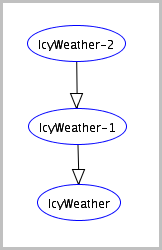
\includegraphics[height=6cm]{img/part4_4.png}
\end{figure} 


  \section{Meltdown}

  \subsection{Question 1}

You can see the modeled wumpus world by loading file \texttt{wumpusWorld.xml}

  \subsection{Question 2}

\begin{figure}[!ht]
  \centering
  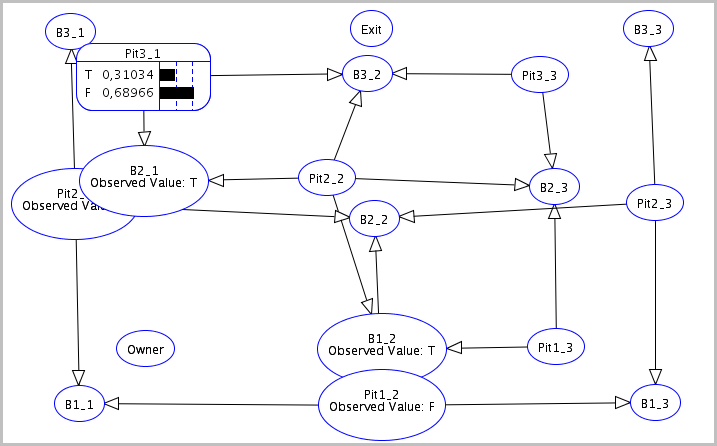
\includegraphics[height=11cm]{img/part5_2.png}
  \caption{Wumpus world : $P(P_{3,1}|known, b)$}
  \label{wumpus5_2}
\end{figure} 

We see the correct answer in the figure \ref{wumpus5_2} : $P(P_{3,1}|known, b) = [0.31, 0.69])$

  \subsection{Question 3}

You can see the modeled wumpus world by loading file \texttt{wumpusWorld2.xml}


\end{document}

